\documentclass[a4paper,12pt]{report}
\usepackage[utf8]{inputenc}
\usepackage[ngerman]{babel}
\usepackage{titlesec}
\usepackage{graphicx}
\graphicspath{ {./images/} }
\usepackage{setspace}
\usepackage{lipsum}
\usepackage{geometry}
\usepackage{tocbibind}
\usepackage{hyperref}
\usepackage{array}
\usepackage{footnote}
\usepackage{natbib}
\bibliographystyle{unsrtnat}
\newcommand{\footcite}[1]{\footnotemark\footnotetext{\cite{#1}}}




\geometry{a4paper, left=25mm, right=25mm, top=30mm, bottom=30mm}

\titleformat{\chapter}{\normalfont\huge}{\thechapter.}{20pt}{\huge\bfseries}
\titleformat{\section}{\normalfont\Large}{\thesection}{12pt}{\Large\bfseries}
\titleformat{\subsection}{\normalfont\large}{\thesubsection}{8pt}{\large\bfseries}

\title{Webbasierte Multiplayer Schach-App}
\author{Jasper Paul Fülle}
\date{24. Mai 2023}

\begin{document}

\begin{titlepage}
    \begin{center}
        \vspace*{1cm}
        
        \Large
        \textbf{Webbasierte Multiplayer Schach-App}
        
        \vspace{0.5cm}
        
        Bachelorarbeit
        
        \vspace{1.5cm}
        
        \normalsize
        vorgelegt von\\
        Jasper Paul Fülle\\
        Matrikelnummer 3367654
        
        \vspace{1cm}
        
        Betreut von\\
        Prof. Dr. Thorsten Thormälen
        
        \vspace{1cm}
        
        \begin{tabular}{>{\raggedright}p{4cm}>{\raggedleft}p{4cm}}
        Studiengang & Wirtschaftsinformatik \\
        \end{tabular}
        
        \vspace{1cm}
        
        \today
        
        \vfill
        
        
        \vspace{0.5cm}
        
        Fachbereich Mathematik und Informatik\\
        Philipps Universität Marburg
    \end{center}
\end{titlepage}

\tableofcontents

\chapter{Einleitung}
    \section{Motivation}
    Schach ist ein traditionsreiches und abwechslungsreiches Brettspiel, deren Ursprung nicht genau bestimmt werden kann. Es wird vermutet, dass das erste schachähnliche Spiel seinen Ursprung in Nordindien um 600 n. Chr. hatte und \textit{Tschaturanga} hieß\footcite{schachgeschichte}.
    Im Laufe der Jahrhunderte hat Schach eine bedeutende Rolle in der Kultur und Geschichte gespielt. So wurde beispielsweise die Schach-WM 1972 eine Art Machtkampf im kalten Krieg zwischen der UdSSR, welche den damaligen Schach dominierten, und der USA\footcite{bobby}.
    Schach bleibt bis heute ein beliebtes Spiel, welches 2020 durch die Netflix Serie \textit{Damengambit} und 2022 durch den Betrugsvorwurf von Magnus Carlsen an seinen 19-jährigen Gegner Hans Niemann\footcite{schachskandal} eine breitere Aufmerksamkeit erhielt (siehe Abbildung \ref{fig:Schachinteresse}). 
     Darüber hinaus hat Schach im digitalen Zeitalter eine neue Popularität erreicht. Online-Schachplattformen wie chess.com verzeichnen Milliarden von Live-Partien\footcite{chesscom3}, während Schach Live-Streams auf Plattformen wie Twitch Millionen von Followern anziehen.
     
Die Entwicklung einer webbasierten Multiplayer-Schach-App bietet eine einzigartige Gelegenheit, ein traditionsreiches und beliebtes Spiel in das digitale Zeitalter zu bringen. Meine Motivation für diese Arbeit besteht darin, eine App zu entwickeln, die die Grundlagen einer Schach-App enthält und gleichzeitig eine solide Basis für zukünftige Erweiterungen und Verbesserungen bietet. Insbesondere plane ich, innovative Funktionen zu integrieren, die bislang in den gängigen Schach-Apps nicht vorhanden sind, wie z.B. die Möglichkeit, unterschiedliche Schachfiguren und -bretter als Belohnungen freizuschalten oder mit Freunden eine Gruppe zu gründen, welche in einer Liga auf- und absteigen kann. Durch die Entwicklung einer Schach-App mit neuen Funktionalitäten kann ich dazu beitragen, die Popularität von Schach zu steigern und vor allem das Spiel einem breiteren Publikum zugänglich zu machen.
    \section{Zielsetzung}
    Diese Bachelorarbeit hat das Ziel eine Schach-App zu entwerfen und zu implementieren, die eine intuitive User Experience und ein ansprechendes User Interface mit vielen nützlichen Funktionen beinhaltet.
    
    User Experience (\textit{UX}) bezieht sich darauf wie ein Nutzer sich auf einer Anwendung bewegt und wie einfach und angenehm es für den Nutzer ist, die Funktionen der Anwendung zu verwenden.
    
    Das User Interface (\textit{UI}) beschäftigt sich mit der visuellen und interaktiven Gestaltung von Benutzeroberflächen. Es umfasst die Gestaltung von Buttons, Formularen und anderen visuellen Komponenten, sowie das Feedback dieser Komponenten, wie zum Beispiel die Rückmeldung eines fehlgeschlagenen Logins.
    Zusammengefasst beschäftigt sich UX damit, wie man eine Anwendung verwendet und UI damit, wie die Benutzeroberfläche der Anwendung aussieht.\footcite{webdesign}
        Funktionen der Schach-App sind unter anderem das Registrieren und Einloggen, das Versenden, Annehmen und Ablehnen von Freundschaftsanfragen, das Zuschauen bei laufenden Spielen, das Herausfordern von Freunden zu Schachspielen und natürlich das Spielen von Schachpartien mit verschiedenen Einstellungsmöglichkeiten der Schach Uhren und einem Chat selbst.
    Dabei wird besonderer Wert auf die Verwendung moderner Web-Technologien wie React, Node.js, Socket.IO, Redis und PostgeSQL gelegt, um eine optimale Benutzererfahrung und Skalierbarkeit zu gewährleisten. Darüber hinaus soll die Arbeit einen Überblick über die technischen Herausforderungen und Lösungen im Zusammenhang mit der Implementierung einer solchen Schach-App bieten.
    
    \section{Aufbau der Arbeit}
Diese Bachelorarbeit gliedert sich in sechs Hauptkapitel, die jeweils unterschiedliche Aspekte der Entwicklung und Implementierung der Schach-App behandeln.

Im ersten Kapitel, der \textit{Einleitung}, werden die Motivation für die Entwicklung der Schach-App, die Zielsetzung der Arbeit und der Aufbau der Arbeit selbst vorgestellt.

Das zweite Kapitel, \textit{Theoretische Grundlagen}, erläutert die Grundlagen von Schach als Spiel sowie die verwendeten Web-Technologien wie Node.js, Express, Socket.io, React und PostgreSQL, die für das Verständnis der nachfolgenden Kapitel wichtig sind.

Im dritten Kapitel, \textit{Systemarchitektur}, wird die Gesamtarchitektur der Schach-App beschrieben, einschließlich der Unterteilung in Frontend und Backend, der Datenbankstruktur und der Kommunikation zwischen den verschiedenen Komponenten.

Das vierte Kapitel, \textit{Implementierung}, geht auf die praktische Umsetzung der Schach-App ein, indem es die Entwicklungsprozesse für das Frontend und das Backend sowie die Integration der Datenbanken erläutert.

Das fünfte Kapitel, \textit{Tests und Evaluation}, behandelt die verschiedenen Tests, die durchgeführt wurden, um die Funktionalität, Usability, Performance und Sicherheit der Schach-App zu bewerten.

Im abschließenden sechsten Kapitel, \textit{Fazit und Ausblick}, werden die Ergebnisse der Arbeit zusammengefasst, eventuelle Limitationen diskutiert und mögliche Erweiterungen und Weiterentwicklungen für die Schach-App vorgeschlagen.

Die Arbeit endet mit dem \textit{Anhang}, der zusätzliche Grafiken und die Liste der verwendeten Literatur enthält.
\chapter{Theoretische Grundlagen}
    \section{Schach}
   Schach ist ein strategisches Brettspiel für zwei Spieler, welches auf einem quadratischen Spielfeld mit 64 Feldern gespielt wird. Jeder Spieler beginnt mit 16 Figuren und das Ziel des Spiels ist es, den König des Gegners schachmatt zu setzen, indem man ihn bedroht, ohne dass der Gegner den Angriff verhindern kann. 
   
   Wie sich welche Figuren bewegen und andere Figuren schlagen erkläre ich nicht explizit, lediglich zwei Sonderregeln des Schach werde ich genauer erklären, da diese bei der Umsetzung des Spiels gesondert gehandhabt werden müssen.
   
   Die erste ist das so genannte \textit{en passant}-Regel. Dabei ist es einem Bauern möglich einen gegnerischen Bauer diagonal zu schlagen, falls dieser zwei Felder gezogen ist und nun auf der gleichen Höhe wie der eigene Bauer steht (siehe Abbildung \ref{fig:en-passant}).
   
   Die zweite Zusatzregel ist die \textit{Bauernumwandlung}. Sie besagt, dass falls ein Bauer die gegnerische Grundreihe erreicht, dieser Bauer in eine Dame, einen Springer, einen Turm oder einen Läufer umgewandelt werden kann (siehe Abbildung \ref{fig:promotion}).
    \section{Web-Technologien}
        \subsection{Node.js und Express}
        \subsection{Socket.io}
        \subsection{React}
        \subsection{PostgreSQL}

\chapter{Systemarchitektur}
Die Anwendung ist in zwei Hauptkomponenten unterteilt: das Frontend und das Backend. Das Frontend ist für die Darstellung der Benutzeroberfläche und die Interaktion mit dem Benutzer verantwortlich, während das Backend die Spiellogik, die Verwaltung der Benutzerdaten und die Echtzeit-Kommunikation zwischen den Spielern steuert.

Die Anwendung verwendet moderne Web-Technologien, um eine reaktive und benutzerfreundliche Oberfläche zu schaffen. Das Frontend basiert auf dem React-Framework\footcite{react}, das es ermöglicht, wiederverwendbare Komponenten zu entwickeln und den Anwendungsstatus effizient zu verwalten. Das User-Interface basiert auf Chakra UI\footcite{chakraui}, einem modernen und flexiblen Komponenten-Bibliothekssystem, das die Entwicklung von responsiven und zugänglichen Benutzeroberflächen erleichtert. Die Benutzerführung und die Kommunikation zwischen den React-Komponenten sind so gestaltet, dass sie eine nahtlose und intuitive Benutzererfahrung bieten.

Auf der Backend-Seite wird Node.js\footcite{nodejs} mit dem Express-Framework verwendet, um einen leistungsstarken und skalierbaren Server bereitzustellen. Die API-Endpunkte und die Kommunikation mittels WebSockets is so konzipiert, dass sie den Anforderungen der verschiedenen Frontend-Komponenten gerecht werden und die Kommunikation zwischen Frontend und Backend erleichtern. Die Echtzeit-Kommunikation zwischen den Spielern wird mit Hilfe von Socket.io\footcite{socketio} ermöglicht, einer Bibliothek, die bidirektionale Kommunikation über WebSockets unterstützt. Für die Speicherung und Verwaltung der Benutzerdaten zum Anmelden wird eine PostgreSQL\footcite{postgresql}-Datenbank verwendet, die aufgrund ihrer Leistungsfähigkeit und Flexibilität ausgewählt wurde. Freundeslisten und Daten aktiver Spiele werden in einer Redis\footcite{redis}-Datenbank gespeichert, die sich durch hohe Leistung und niedrige Latenz auszeichnet, insbesondere bei Lese- und Schreibvorgängen. Redis, eine In-Memory-Datenstruktur, eignet sich ideal für Anwendungen, bei denen schnelle Zugriffszeiten und Skalierbarkeit wichtig sind. Die Kombination von PostgreSQL und Redis ermöglicht eine effiziente Verwaltung sowohl persistenter als auch flüchtiger Daten und fördert eine optimale Benutzererfahrung.
    \section{Frontend}
        \subsection{React-Komponenten}
    
        \subsection{Benutzerführung}
        \subsection{Kommunikation mit dem Backend}
    \section{Backend}
        \subsection{API-Endpunkte}
        \subsection{Datenbankstruktur}
        		\subsubsection{PostgreSQL}
        		\subsubsection{Redis}
        \subsection{Echtzeit-Kommunikation}

\chapter{Implementierung}
    \section{Frontend-Entwicklung}
    \section{Backend-Entwicklung}
    \section{Datenbank-Integration}

\chapter{Tests und Evaluation}
    \section{Funktionalitätstests}
    \section{Usability-Tests}
    \section{Performancetests}
    \section{Sicherheitstests}

\chapter{Fazit und Ausblick}
    \section{Zusammenfassung der Ergebnisse}
    \section{Limitationen}
    \section{Potenzielle Erweiterungen und Weiterentwicklung}

\appendix

\listoffigures
\begin{figure}[ht]
\raggedleft
  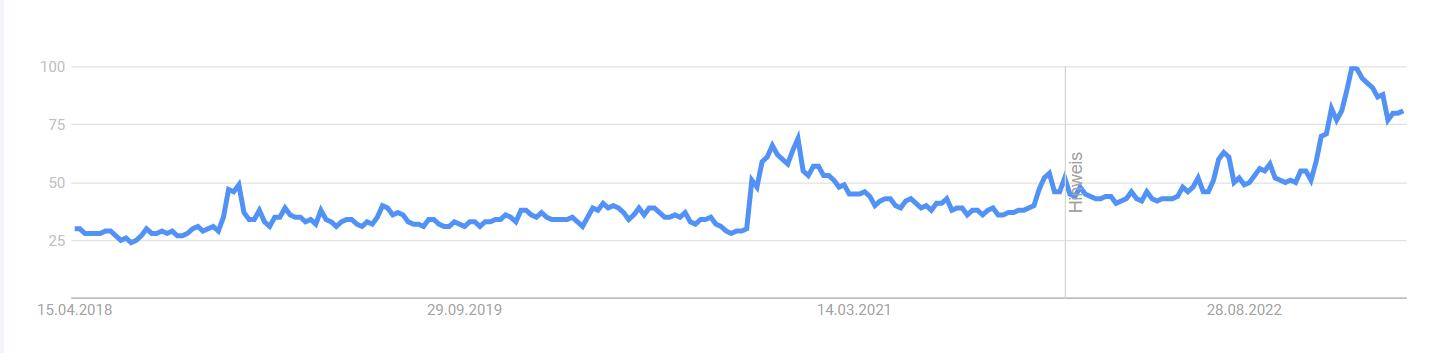
\includegraphics[width=160mm]{Schachentwicklung.jpg}
    \footnotesize\sffamily\textbf{Quelle:} \url{https://trends.google.de/}
  \caption{Relatives Suchinteresse des Wortes \textit{Chess} auf Google in den letzten 5 Jahren.}
  \label{fig:Schachinteresse}
\end{figure}
  
  \begin{figure}[ht]
\raggedleft
  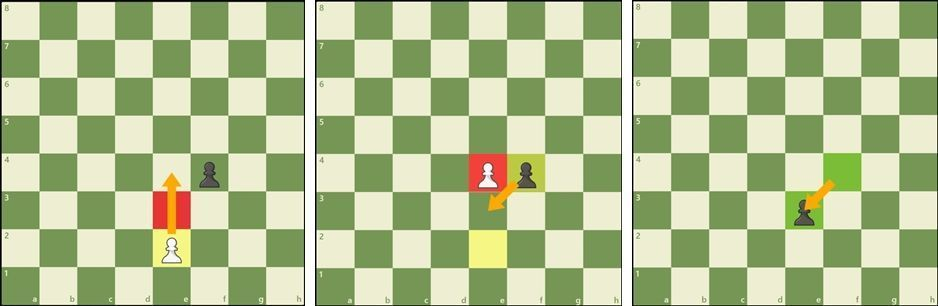
\includegraphics[width=160mm]{en-passant.jpeg}
    \footnotesize\sffamily\textbf{Quelle:} \url{https://www.chess.com/de/schachregeln}
  \caption{Die Zusatzregel \textit{en passant}}
  \label{fig:en-passant}
\end{figure}

  \begin{figure}[ht]
\centering
  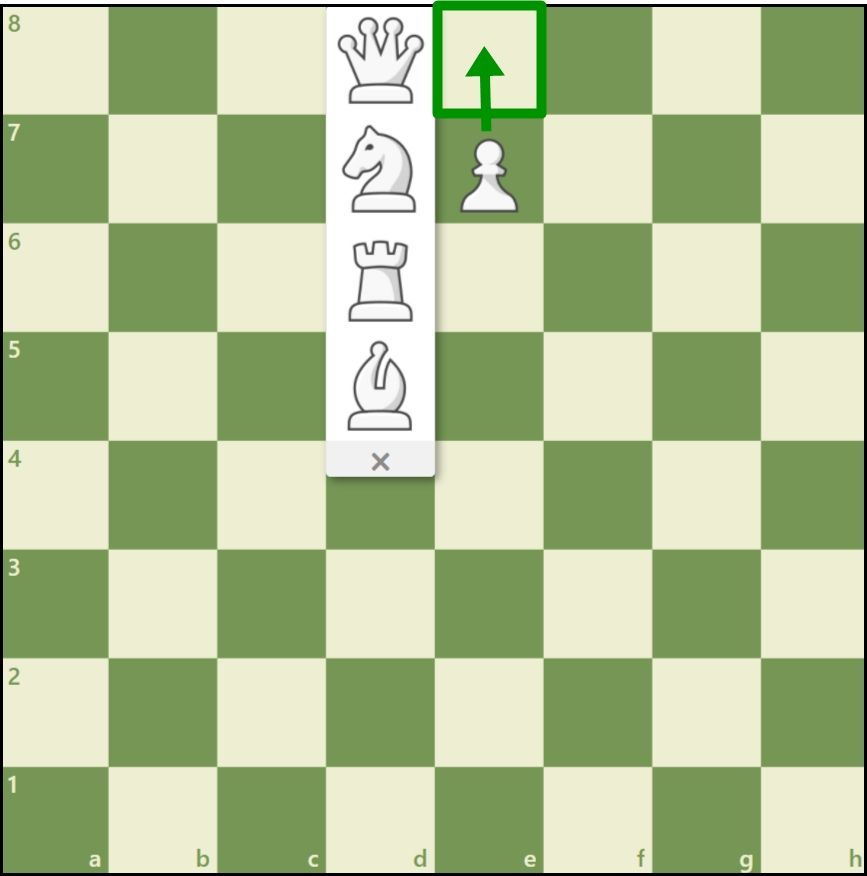
\includegraphics[height=80mm]{promotion.jpeg}
   
   
\raggedleft
    \footnotesize\sffamily\textbf{Quelle:} \url{https://www.chess.com/de/schachregeln}
  \caption{Die Zusatzregel \textit{Bauernumwandlung}}
  \label{fig:promotion}
\end{figure}



\bibliography{Bibliography}

\end{document}

